%-------------------------
% Resume in Latex
% Author : Jake Gutierrez
% Based off of: https://github.com/sb2nov/resume
% License : MIT
%------------------------

\documentclass[letterpaper,11pt]{article}

\usepackage{latexsym}
\usepackage[empty]{fullpage}
\usepackage{titlesec}
\usepackage{marvosym}
\usepackage[usenames,dvipsnames]{color}
\usepackage{verbatim}
\usepackage{enumitem}
\usepackage[hidelinks]{hyperref}
\usepackage{fancyhdr}
\usepackage[english]{babel}
\usepackage{tabularx}
\usepackage{fontawesome5}
\usepackage{multicol}
\usepackage{wasysym}
\usepackage{lastpage}


\usepackage{tikz}
\usepackage{graphicx}

\setlength{\multicolsep}{-3.0pt}
\setlength{\columnsep}{-1pt}
\input{glyphtounicode}
\usepackage{fontawesome5}

\newcommand{\portfoliosymbol}{\faFolderOpen\hspace{-.1em}\faBriefcase}

\pagenumbering{arabic}



%----------FONT OPTIONS----------
% sans-serif
% \usepackage[sfdefault]{FiraSans}
% \usepackage[sfdefault]{roboto}
% \usepackage[sfdefault]{noto-sans}
% \usepackage[default]{sourcesanspro}

% serif
% \usepackage{CormorantGaramond}
% \usepackage{charter}


\pagestyle{fancy}
\fancyhf{} % clear all header and footer fields
\fancyfoot{}
\renewcommand{\headrulewidth}{0pt}
\renewcommand{\footrulewidth}{0pt}

% Adjust margins
\addtolength{\oddsidemargin}{-0.6in}
\addtolength{\evensidemargin}{-0.5in}
\addtolength{\textwidth}{1.19in}
\addtolength{\topmargin}{-.7in}
\addtolength{\textheight}{1.4in}

\urlstyle{same}

\raggedbottom
\raggedright
\setlength{\tabcolsep}{0in}

% Sections formatting
\titleformat{\section}{
  \vspace{-4pt}\scshape\raggedright\large\bfseries
}{}{0em}{}[\color{black}\titlerule \vspace{-5pt}]

% Ensure that generate pdf is machine readable/ATS parsable
\pdfgentounicode=1

%-------------------------
% Custom commands
\newcommand{\resumeItem}[1]{
  \item\small{
    {#1 \vspace{-2pt}}
  }
}

\newcommand{\classesList}[4]{
    \item\small{
        {#1 #2 #3 #4 \vspace{-2pt}}
  }
}

\newcommand{\resumeSubheading}[4]{
  \vspace{-2pt}\item
    \begin{tabular*}{1.0\textwidth}[t]{l@{\extracolsep{\fill}}r}
      \textbf{#1} & \textbf{\small #2} \\
      \textit{\small#3} & \textit{\small #4} \\
    \end{tabular*}\vspace{-7pt}
}

\newcommand{\resumeSubSubheading}[2]{
    \item
    \begin{tabular*}{0.97\textwidth}{l@{\extracolsep{\fill}}r}
      \textit{\small#1} & \textit{\small #2} \\
    \end{tabular*}\vspace{-7pt}
}

\newcommand{\resumeProjectHeading}[2]{
    \item
    \begin{tabular*}{1.001\textwidth}{l@{\extracolsep{\fill}}r}
      \small#1 & \textbf{\small #2}\\
    \end{tabular*}\vspace{-7pt}
}

\newcommand{\resumeSubItem}[1]{\resumeItem{#1}\vspace{-4pt}}

\renewcommand\labelitemi{$\vcenter{\hbox{\tiny$\bullet$}}$}
\renewcommand\labelitemii{$\vcenter{\hbox{\tiny$\bullet$}}$}

\newcommand{\resumeSubHeadingListStart}{\begin{itemize}[leftmargin=0.0in, label={}]}
\newcommand{\resumeSubHeadingListEnd}{\end{itemize}}
\newcommand{\resumeItemListStart}{\begin{itemize}}
\newcommand{\resumeItemListEnd}{\end{itemize}\vspace{-5pt}}

%-------------------------------------------
%%%%%%  RESUME STARTS HERE  %%%%%%%%%%%%%%%%%%%%%%%%%%%%


\begin{document}

%----------HEADING----------
% \begin{tabular*}{\textwidth}{l@{\extracolsep{\fill}}r}
%   \textbf{\href{http://sourabhbajaj.com/}{\Large Sourabh Bajaj}} & Email : \href{mailto:sourabh@sourabhbajaj.com}{sourabh@sourabhbajaj.com}\\
%   \href{http://sourabhbajaj.com/}{http://www.sourabhbajaj.com} & Mobile : +1-123-456-7890 \\
% \end{tabular*}
\parbox{3.0cm}{%

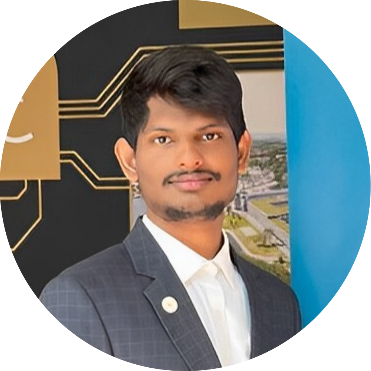
\includegraphics[width=2.7cm,clip]{images/resume_pic_m.png}}
}
\parbox{\dimexpr\linewidth-3.8cm\relax}{
\vspace{-20pt}
\begin{tabularx}{\linewidth}{L r} \\
    {\Huge \scshape  Venkata Sai Yakkshit Reddy Asodi}~
    \href{https://www.cedzlabs.com/yakkshit}{\vspace{1pt}}\\
      \\ \vspace{1pt}
     \small \raisebox{-0.1\height}\faPhone\ +46 0793550685 ~ \href{mailto:saiyakkshit2001@gmail.com}{\raisebox{-0.2\height}\faEnvelope\  {saiyakkshit2001@gmail.com}} ~ 
    \href{https://linkedin.com/in/yakkshit/}{\raisebox{-0.2\height}\faLinkedin\ {yakkshit}}  ~
    \href{https://yakkshit.com/}{\raisebox{-0.2\height}\faGlobe\ {yakkshit.com}}  ~
    \href{https://github.com/yakkshit}{\raisebox{-0.2\height}\faGithub{ yakkshit}}
    \vspace{-8pt}
    
\end{tabularx}
}




\vspace{-10pt}

%-----------------------------------
\href{https://www.yakkshit.com/#details}{\section{Summary \faLink}
I am a \textbf{Software Developer} with a passion for building high-quality software. I have experience in Web Development and have contributed to the product lifecycle, from requirements analysis to deployment. I have a strong understanding of authentication and authorization, and I effectively manage automation, networking, and logs using tools such as Bash Scripting in Linux, 
Python programming, 
AWS CLI. 
I have hands-on experience with 
NextJs,
Azure,
Spring Boots,
Postgres, infrastructure as code, and GitHub version control. I have extensive experience in implementing professional practices such as Agile methodologies. In recent times I have also contributed to Micro K8s clusters and Kubernetes.}


%-----------PROGRAMMING SKILLS-----------
\section{\href{https://www.linkedin.com/in/yakkshit/details/skills/}{Technical Skills} \faLink}
 \begin{itemize}[leftmargin=0.15in, label={}]
    \small{\item{
     \textbf{Deployment/Automation/templating tools - }{Jenkins, Docker, Bash Scripting, Github, Bitbucket/Gitlab.} \\
     \textbf{Frameworks - }{Django, TensorFlow.}\\
     \textbf{Languages - }{ Python, Java, C++ , C, HTML, CSS, JS, PHP, SQL, TypeScript.}\\
    }}
 \end{itemize}
%-----------EXPERIENCE-----------
\section{\href{https://www.linkedin.com/in/yakkshit/}{Professional Experience  \faLink}}
  \resumeSubHeadingListStart
  \resumeSubheading
      {\large BetaTesting.Inc}{Jan 2023 -- June 2023}
      {Application Tester}{\faMapMarker Remote}\\
      \vspace{10pt}
      % \textbf{Responsibilities:}
      % Conducted beta testing for a new application, developed a test plan, executed test cases, and reported 25+ critical bugs to the development team, reducing the overall bug rate by 40\%\. Used various testing methods such as functional, load, security, compatibility, usability, and automated testing to enhance application performance. Utilized tracing method and performance analysis in the development environment to visualize and analyze the application.
      \textbf{Responsibilities :}
      \resumeItemListStart
      \vspace{-10pt}
      \resumeItem{Conducted beta testing for a new application, developed a test plan, executed test cases, and reported 25+ critical bugs to the development team, reducing the overall bug rate by 40\%\. Used various testing methods such as functional, load, security, compatibility, usability, and automated testing to enhance application performance. Utilized tracing method and performance analysis in the development environment to visualize and analyze the application.}
      %   \resumeItem{Conducted beta testing for new Application by developing a comprehensive test plan, executing test cases, and identifying/reporting 25+ critical bugs to the development team; reduced the overall bug rate by 40\%.}
      %   \resumeItem{I have used the following testing methods Functional, Load, Security, Compatibility, Usability, Automated Testing to enhance the performance of the Application.}
      %   \resumeItem{Utilizing Tracing method as the development environment to visualize and analyze the application and Leveraging performance analysis.}
    \resumeItemListEnd
    \vspace{-3pt}
    \textbf{Environment:}\emph{Bug reporting, debugging, problem-solving, collaboration, Appium.}

    \resumeSubheading
      {CEDZLABS.COM}{May 2021 -- Dec 2022}
      {FullStack Engineer}{\faMapMarker Remote}\\
      \vspace{10pt}
      % \textbf{Responsibilities : }Created and maintained websites and web applications using multiple programming languages and technologies. Utilized Django framework and RESTful APIs to improve functionality and interactivity of websites. Monitored website performance through Google Search Console, Google Analytics, and Firebase Performance SDK.
\textbf{Responsibilities : }
        \vspace{-10pt}
      \resumeItemListStart
      \resumeItem{Created and maintained websites and web applications using multiple programming languages and technologies. Utilized Django framework and RESTful APIs to improve functionality and interactivity of websites. Monitored website performance through Google Search Console, Google Analytics, and Firebase Performance SDK.}
%         \resumeItem{Utilized a range of programming languages and technologies to create and maintain websites and web applications.}
%         \resumeItem{Implemented the Django framework to enhance the functionality and interactivity of websites.}
%         \resumeItem{Integrated various RESTful APIs to enhance the functionality and features of websites.}
%         \resumeItem{Monitored website performance using Google Search Console, Google Analytics, and Firebase Performance SDK.}\\
        \vspace{-3pt}
      \resumeItemListEnd
\textbf{Environment:}\emph{HTML, CSS, JavaScript, Node.js, SQL databases, Django, Google Search Console, Google Analytics, Firebase Performance SDK.}
  
    \resumeSubheading
      {VERZEO.INC}{Aug 2020 -- Mar 2021}
      {AI Engineer Intern}{ \faMapMarker Remote}\\
      % \textbf{Responsibilities : }Implemented a face mask detection system using Matlab, TensorFlow, OpenCV, and deep learning techniques on a provided dataset. Integrated the model into a real-time system using OpenCV's computer vision capabilities and conducted thorough testing to ensure its precision and reliability. Used Python, TensorFlow, OpenCV, Keras, and deep learning.
      \vspace{10pt}

\textbf{Responsibilities : }
      \vspace{-10pt}
      \resumeItemListStart
      \resumeItem{Implemented a face mask detection system using Matlab, TensorFlow, OpenCV, and deep learning techniques on a provided dataset. Integrated the model into a real-time system using OpenCV's computer vision capabilities and conducted thorough testing to ensure its precision and reliability. Used Python, TensorFlow, OpenCV, Keras, and deep learning.}
%         \resumeItem{Utilized Matlab, TensorFlow, OpenCV, and deep learning techniques to implement the project, working with a provided dataset.}
%         \resumeItem{Integrated the trained model into a real-time face mask detection system using the OpenCV library and its computer vision capabilities.}
%         \resumeItem{Conducted comprehensive testing to ensure the precision and reliability of the face mask detection system.}
%         \\
      \resumeItemListEnd
    \vspace{-3pt}
\textbf{Environment:}\emph{Python, TensorFlow, OpenCV, Keras, Deep learning.}
\resumeSubHeadingListEnd

%-----------PROJECTS-----------
\section{\href{https://www.yakkshit.com/#project-1}{Projects} }
    \resumeSubHeadingListStart

%---------------------------------------------------------------------------
                
                            % Embedded systems

                            
% -----------------------------------------------------------------------------


% \resumeProjectHeading
%           {\textbf{\href{https://github.com/yakkshit/air}{CO2 monitoring system}} $|$ \emph{CI/CD, Embedded Systems \faGithub}}{March 2023}\\
%           \vspace{9pt}
%           \vspace{-8pt}
%           \resumeItemListStart
%           \resumeItem{I developed an air quality monitor with particle matter (PM1, PM12.5, PM4, PM10), eCO2, and TVOC monitoring, as well as MQTT connectivity. The project uses a LILYGO TTGO T-Display ESP32 microcontroller, a Particulate Matter Sensor SPS30, and an SGP30 Air Quality Sensor. The sensors are connected to the I2C bus (pin 21 and 22). The project also depends on the Button2, PubSubClient, WiFiClientSecure, and Arduinosps libraries. }
          
% %             % \resumeItem{I have used Unity Engine for the development of the 2048 3D game.}
% %             % \resumeItem{The script was return in c\#\ .}
% %             % \resumeItem{The Asserts being imported from Unity store.}
% %             % \resumeItem{The game is being deployed in both Web and Android.}
            
%           \resumeItemListEnd 
%           \textbf{Tools:}\emph{
%                                 c++, Sensor interfacing, MQTT communication, Arduino, Data visualization.}

%---------------------------------------------------------------------------
                
                            % Bachlore Thesis
% -----------------------------------------------------------------------------

 \resumeProjectHeading
          {\textbf{\href{https://www.yakkshit.com/#project-1}{Analysis of Webxr and Arcore}} $|$ \emph{Bachelor Thesis \faGithub}}{June 2023}\\
          \vspace{9pt}
          \vspace{-8pt}
          \resumeItemListStart
            \resumeItem{Developed an Android and web AR application using Firebase, ARCore API, and Three.js. Created a 3D model in Blender deployed to the cloud. Conducted hardware tests and utilized machine learning (KNN, Random Forest) for analysis. Proficient in system tracing tools like TensorFlow Profiler, strace, and perf for performance optimization.}
          \resumeItemListEnd 
          \textbf{Tools:}\emph{
                                Kotlin / Java, Threejs , Webxr, Machine Learning, Gui, hardware Testing, Data analysis.}

 
%---------------------------------------------------------------------------
                
                            % 2048 Game
% -----------------------------------------------------------------------------

 % \resumeProjectHeading
 %          {\textbf{\href{https://github.com/yakkshit/2048-3d-master.git}{2048 3d game}} $|$ \emph{CI/CD, Unity \faGithub}}{March 2023}\\
 %          \vspace{9pt}
 %          \vspace{-8pt}
 %          \resumeItemListStart
 %            \resumeItem{I used Unity Engine to develop the 2048 3D game, with the script written in C#. The assets were imported from the Unity store, and the game is available on both web and Android platforms.}
 %            % \resumeItem{The script was return in c\#\ .}
 %            % \resumeItem{The Asserts being imported from Unity store.}
 %            % \resumeItem{The game is being deployed in both Web and Android.}
 %          \resumeItemListEnd 
 %          \textbf{Tools:}\emph{
 %                                Unity, C\#\ , WebGL, android, continuous integration.}

%---------------------------------------------------------------------------
                
                            % Azure DEvops
% -----------------------------------------------------------------------------


        % \resumeProjectHeading
        % {\textbf{\herf{}{Azure DevOps}} $|$ \emph{CI/CD, Azure.}}{March 2023}\\
        % \vspace{6pt}
        % \textbf{Description:}
        % \vspace{-5pt}
        %   \resumeItemListStart
        %   \resumeItem{Automated software development and deployment, resulting in improved quality and faster deployment of new features and bug fixes. Overcame challenges by learning Azure DevOps Services, integrating them with existing tools, and scheduling efficient deployments. Implemented a comprehensive approach with a training plan, custom integration, and streamlined deployment process. Project aimed to improve software quality and reduce deployment time.}

        
          % \resumeItem{Automated the software development and deployment process, resulting in improved software quality and reduced time for deploying new features and bug fixes.}
          % \resumeItem{Successfully tackled challenges that involved learning how to use Azure DevOps Services, integrating them with our existing development tools, and effectively scheduling deployments to production.}
          % \resumeItem{Implemented a comprehensive approach, including creating a training plan for the team on Azure DevOps Services, developing a custom integration with existing development tools, and establishing an efficient process for scheduling deployments to production.}
          % \resumeItem{The project was done to improved software quality and reduced time for deploying new features and bug fixes.}
          % \resumeItemListEnd 
          % \textbf{Tools:}\emph{ \href{https://yakkshit.com}{AWS KMS, S3, encryption, decryption, unique key, IAM, secure files, web development, Nextjs, React.}}
          
%---------------------------------------------------------------------------
                
                            % CI/CD Gerrit code review
% -----------------------------------------------------------------------------

%       \resumeProjectHeading
%       {\href{https://review.gerrithub.io/admin/repos/saiyakkshit/py-chess-svg,general}{\textbf{Deploying an Application using Gerrit}} $|$ \emph{CI/CD, Visual Studio Code \faGithub}}
%       {March 2023}\\
%           \vspace{6pt}
%           \textbf{Description:}
%           \vspace{-5pt}
%           \resumeItemListStart
%           \resumeItem{Implemented Zuul CI with Gerrit Code Review for efficient code review and integration. Developed a Python project integrated with Zuul, incorporating third-party dependencies to generate SVG images. Extended the project with Bazel integration, creating a Python wheel file, performing unit tests, and utilizing Zuul for artifact management and coverage reports.}

      
%     % \resumeItem{
%     % % \href{https://review.gerrithub.io/admin/repos/saiyakkshit/py-chess-svg,general}
%     % Implemented Zuul CI with Gerrit Code Review, utilizing Zuul concepts and project gating for efficient code review and integration process.
%     % }
%     %         \resumeItem{
%     %         % \href{https://review.gerrithub.io/admin/repos/saiyakkshit/py-chess-svg,general}{
%     %         Developed a Python project integrated with Zuul, incorporating third-party dependencies such as python-chess to generate SVG images based on input moves.}
%     %         \resumeItem{
%     %         % \href{https://review.gerrithub.io/admin/repos/saiyakkshit/py-chess-svg,general}{
            
%     %         Extended the project with Bazel integration, creating a Python wheel file, performing unit tests, and utilizing Zuul for artifact management and coverage reports.}
    
%           \resumeItemListEnd 
%           \textbf{Tools:}\emph{\href{https://review.gerrithub.io/admin/repos/saiyakkshit/py-chess-svg,general}{
% Zuul CI, Gerrit Code Review, Bazel, unit tests, Jtest, coverage reports.}}

%         \vspace{-18pt}

%

%---------------------------------------------------------------------------
                
                            % Linux articture
                            
% -----------------------------------------------------------------------------
%           \resumeProjectHeading
%           {\textbf{\href{https://github.com/saiyakkshit?tab=repositories}{Debian Contents Tool
% }} $|$ \emph{python, Linux \faGithub}}{January 2023}\\
%           \vspace{6pt}
%           \textbf{Description:}
%            \vspace{-5pt}
%           \resumeItemListStart
%             \resumeItem{Created a Python tool that downloads and analyzes the compressed Contents file for a Debian architecture, displaying statistics on the top 10 packages with the most associated files. The project followed Python's best practices, including comments, unit tests, and adherence to the PEP 8 style guide. The work was organized in a local Git repository, allowing for progress tracking, collaboration, and data parsing using JSON from the Debian mirror. Regular expressions were employed to extract package information from the Contents file using the re.search() and re.findall() methods.}
          
%             % \resumeItem{Developed a Python command line tool that downloads the compressed Contents file associated with a Debian architecture and outputs the statistics of the top 10 packages that have the most files associated with them.}
%             % \resumeItem{Followed Python's best practices in my solution, including using comments to explain my code, unit tests to verify its functionality, and following the PEP 8 style guide.}
%             % \resumeItem{Organized my work in a local Git repository, which allowed me to track my progress, collaborate with others, and store and parse data from the Debian mirror using JSON.}    
%             % \resumeItem{Used regular expressions to extract package information from the Contents file using the re.search() and re.findall() methods.}
%           \resumeItemListEnd 
%           \textbf{Tools:}\emph{Python, Unit testing, Git, JSON, Regular expressions.}



% ---------------------------------------------------------------------------
                
                            % Portfolio
                            
% -----------------------------------------------------------------------------
          
          \resumeProjectHeading
          {\href{https://yakkshit.com}{\textbf{AWS Hosting Deployment, Monitoring, and Serverless Functions }} $|$ \emph{NextJS, AWS CLI} \faGithub}{January 2023}\\
          \vspace{6pt}
          \textbf{Description:} 
          \vspace{-5pt}
          \resumeItemListStart
            \resumeItem{\href{https://yakkshit.com}{Designed and implemented a secure file encryption/decryption system using AWS KMS and S3, with access controls enforced through IAM.}}
            \resumeItem{\href{https://yakkshit.com}{Built and deployed a scalable and efficient website using NextJS, threeJS, and AWS services (S3, Lambda), leveraging GitHub Actions for automated deployment and builds, and monitored website performance using AWS CloudWatch. Additionally, utilized the Storybook component library to enhance the design and development process, and hosted the website on GitHub Pages for easy access and visibility.}}
            \resumeItem{\href{https://yakkshit.com}{Designed and developed a visually appealing and user-friendly UI/UX for my portfolio website using Storybook, Figma and React, with a component-centric approach that enhances the user experience.}}
          \resumeItemListEnd
          \vspace{-2pt}
          \textbf{Tools:}\emph{ \href{https://yakkshit.com}{AWS KMS, S3, encryption, decryption, unique key, IAM, secure files, web development, Nextjs, React.}}




%---------------------------------------------------------------------------
                
                            % fire walls 
% -----------------------------------------------------------------------------

\resumeProjectHeading
          {\textbf{\href{https://github.com/saiyakkshit?tab=repositories}{Networking and Firewalls}} $|$ \emph{Bash, Ubuntu \faGithub}}{November 2022}\\
          \vspace{6pt}
          \textbf{Description:}
           \vspace{-5pt}
          \resumeItemListStart
          \resumeItem{Established communication between networked devices using bash scripting and Ubuntu. Employed HTTP requests for data transfer and set up firewall rules for secure communication. Updated firewall rules to establish a secure connection between client and server.}
%             % \resumeItem{Established communication between networked devices using bash scripting and Ubuntu.}
%             % \resumeItem{Employed HTTP requests for data transfer and set up firewall rules to ensure secure communication.}
%             % \resumeItem{Updated firewall rules to establish a secured connection between client and server.}           
          \resumeItemListEnd 
          \textbf{Tools:}\emph{Bash scripting,
Ubuntu OS,
C Programming,
HTTP requests, Network Security,
Firewall rules.}

% % ---------------------------------------------------------------------------
                
% %                             Fall Detection
% % -----------------------------------------------------------------------------
%           \resumeProjectHeading          {\textbf{\href{https://github.com/yakkshit/Fall-Detection-Via-Camera-2D.git}{Fall Detection system}} $|$ \emph{ML, VS code \faGithub}}{September 2022}\\
%           \vspace{6pt}
%           \textbf{Description:}
         
%           \vspace{-8pt}
%           \resumeItemListStart
%           \resumeItem{Developed a fall detection algorithm using Yolo v4 and OpenCV with 95\%\ accuracy. Trained on over 10,000 images of falls and non-falls. Built a web app with Django framework for viewing videos of falls and confirming them. Sent SMS notifications to guardians within 10 seconds of fall detection via Twilio's API.}
%             % \resumeItem{ Developed a fall detection algorithm using Yolo v4 and OpenCV, achieving an accuracy of 95\%.}
%             % \resumeItem{The fall detection algorithm was trained on a dataset of over 10,000 images of falls and non-falls.}
%             % \resumeItem{Built a web application using Django frame work, which allows users to view video recordings of falls and confirm whether or not a fall has occurred.}
%             % \resumeItem{Sent SMS notifications to guardians within 10 seconds of a fall being detected using Twilio's API.}
%           \resumeItemListEnd 
%           \textbf{Tools:}\emph{
% Computer vision, Machine learning, Python, Django.}


%---------------------------------------------------------------------------
                
                            % Gcp Devops
% -----------------------------------------------------------------------------

          % \resumeProjectHeading
          % {\textbf{\href{https://www.cloudskillsboost.google/public_profiles/6bf05c97-e7a5-48b7-bd37-03938dae9743/badges/2357183}{DevOps Essentials in Google Cloud}} $|$ \emph{CI/CD, Google Cloud Console}}{June 2022}\\
          % \vspace{6pt}
          % \textbf{Description:}
          % \vspace{-5pt}
          % \resumeItemListStart
          %   \resumeItem{Utilized Cloud Source Repositories, Kubernetes Engine, Load Balancers, and troubleshooting workloads on GKE to improve DevOps practices in GCP.}
          %   \resumeItem{Created Kubernetes clusters and used Docker for containerization for cloud repositories with Git for version control.}
          %   \resumeItem{Managed deployments using Kubernetes Engine, scaling and managing containers for common scenarios.}
          %   \resumeItem{Deployed Kubernetes Load Balancer Service with Terraform, setting up a Kubernetes cluster and deploying Nginx service on it.}
          %   \resumeItem{Deployed using continuous integration and configured a continuous delivery pipeline using Jenkins on Kubernetes Engine.}
          % \resumeItemListEnd 
          % \vspace{-12pt}
          % \textbf{Tools:}\emph{
          %       Terraform, Docker, Kubernetes, iaas, Nginx, Jenkins, DevOps.}
% \vspace{-10pt}

%---------------------------------------------------------------------------
                
                            % Langversation
                            
% -----------------------------------------------------------------------------

    \resumeProjectHeading          {\textbf{\href{https://github.com/saiyakkshit/Langversation}{Langversation}} $|$ \emph{CI/CD, Android Studio \faGithub}}{December 2022}\\
          \vspace{6pt}
          \textbf{Description:}
         
          \vspace{-8pt}
          \resumeItemListStart
          \resumeItem{Langversation is an end-to-end encrypted multilingual chat-based android app developed in Kotlin. XML was used for the front end and Kotlin for the back end of user conversation. FirebaseStorage and FirebaseAuthentication were used for storage and authentication. Ml kit translational API was used for language translation. Firebase Performance SDK and Firebase Crashlytics SDK were used to monitor app performance and crashes.}
            % \resumeItem{ Langversation is a communication, end‑to‑end encrypted multilingual chat‑based android application which was developed in kotlin.}
            % \resumeItem{In the development of user conversation i have used XML as front end and Kotlin for the back end.}
            % \resumeItem{For the storage and authentication which was used in the app was done in FirebaseStorage and FirebaseAuthentication.}
            % \resumeItem{Ml kit translational API which was used to convert from one language to the other.}
            % \resumeItem{The Performance and Crashes of the App was monitered using the Firebase Performance SDK and Firebase Crashlytics SDK.}
          \resumeItemListEnd 
          \textbf{Tools:}\emph{
Kotlin, java, ML kit, Firebase, XML.}


%---------------------------------------------------------------------------
                
                            % End
% -----------------------------------------------------------------------------

%-----------EDUCATION-----------
\section{Education Details  \faGraduationCap   }

% \hfill \textbf{\LARGE 
%  \raisebox{9pt} {Software Developer}}
 
  \resumeSubHeadingListStart
    \resumeSubheading
      {Blekinge Institute of Technology}{Sep. 2022 -- June. 2023}
      {Bachelor of Science in Computer Science}{\faMapMarker Valhallavägen 1, 371 41 Karlskrona.}
  \resumeSubHeadingListEnd
    \vspace{-7pt}
  \resumeSubHeadingListStart
    \resumeSubheading
      {University College Of Engineering Jntuk}{Aug. 2019 -- Jun. 2022}
      {Bachelor of Science in Computer Science}{\faMapMarker Kakinada, AndhraPradesh, India 533003.}
  \resumeSubHeadingListEnd


%------RELEVANT COURSEWORK-------
\section{\href{https://www.linkedin.com/in/yakkshit/details/courses/}{Relevant Coursework} }
    %\resumeSubHeadingListStart
        \begin{multicols}{4}
            \begin{itemize}[itemsep=-4pt, parsep=3pt]
                \item\small Data Structures
                \item Software Methodology
                \item Algorithms Analysis
                \item Database Management
                \item Network Slicing(5G)
                \item Information Technology
                \item RESTful API
                \item distributed systems \\
                \item Kafka
                \item IOT
                \item microservices
                \item System Administration\\
            \end{itemize}
        \end{multicols}
        \vspace*{2.0\multicolsep}
    %\resumeSubHeadingListEnd

%-----------INVOLVEMENT---------------
\section{\href{https://www.linkedin.com/in/yakkshit/details/certifications/}{Certificates / Achivements} \faLink}
            \resumeItemListStart
            \resumeItem{\href{https://portal.certiport.com/Portal/Pages/PrintTranscriptInfo.aspx?action=Cert&id=395&cvid=ej8fNHXiWfEntRn/kBIQHw==}{I have Achieved
                MTA(Microsoft Technical Associate)-Python}}
                \vspace{-2pt}
                \resumeItem{\href{https://drive.google.com/file/d/1dhl67D-8GIbrHul7yOXaZnMi9Wy8rkg4/view}{I have Completed as a AI - Intern at Verzeo.inc}}
                \vspace{-2pt}
                \resumeItem{\href{https://portal.certiport.com/Portal/Pages/PrintTranscriptInfo.aspx?action=Cert&id=398&cvid=QiBkzVlVnojF0hDdRTf01Q==}{I have Achieved
                MTA(Microsoft Technical Associate)-Java}}
                \vspace{-2pt}
                \resumeItem{\href{https://www.cloudskillsboost.google/public_profiles/6bf05c97-e7a5-48b7-bd37-03938dae9743}{I have Achieved a Skill badges at Google Cloud carrier path}}
                \vspace{-2pt}
                \resumeItem{\href{https://www.linkedin.com/in/yakkshit/details/certifications/}{I have Achieved azure Certificates and many other Related to Software Development.}}
                
                
            \resumeItemListEnd
\vspace{-10pt}
%-----------INVOLVEMENT---------------
\section{Leadership / Extracurricular / Contributions}
            \resumeItemListStart
                \vspace{-3pt}\resumeItem{\href{https://cedzlabs.com}{Led a chapter of 30+ members to work towards goals that improve and promote CedzLabs community service, with collaborative environment, academics, and unity.}}\\
                \resumeItem{I contributed to Kubernetes is Developed new functions in the release script to ensure a smooth and error-free release process by checking dependencies, generating release notes for microserves and uploading the final tarball to a remote storage location.}
                % \vspace{-7pt}
                \resumeItem{\href{https://github.com/yakkshit/charm-microk8s/pull/2/files}{I have contributed to adding a new class, MicroK8sClusterUpgradeEvent, to the Micro K8 Cluster and implemented upgrade logic to handle it for performing necessary upgrade logic for the Micro K8s cluster.}}
                \resumeItem{I have extensive experience in implementing professional practices such as Agile methodologies including Scrum and Kanban.}
                
                
            \resumeItemListEnd
    \textbf{Strengths : }\emph{Leadersip skills,
Multitasking, decision making,
Attention to details.
}
\end{document}
